%%%%%%%%%%%%%%%%%%%%%%%%%%%%%%%%%%%%%%%%%%%%%%%%%%%%%%%%%%%%%%%%%%%%%
%
% NOTE: WORK IN PROGRESS
%
% Modification to ACM sample.
% Based on:
% acmsmall-sample.tex, dated 15th July 2010
% This is a sample file for ACM small trim journals
%
% Compilation using 'acmsmall.cls' - version 1.1, Aptara Inc.
% (c) 2010 Association for Computing Machinery (ACM)
%
% Questions/Suggestions/Feedback should be addressed to => "acmtexsupport@aptaracorp.com".
% Users can also go through the FAQs available on the journal's submission webpage.
%
% Steps to compile: latex, bibtex, latex latex
%
% For tracking purposes => this is v1.1 - July 2010
%%%%%%%%%%%%%%%%%%%%%%%%%%%%%%%%%%%%%%%%%%%%%%%%%%%%%%%%%%%%%%%%%%%%%

\documentclass[prodmode,acmtecs]{acmsmall}

\usepackage{draftcopy}

\usepackage{graphicx}
\usepackage{type1cm}
\usepackage{eso-pic}
\usepackage{color}

% Package to generate and customize Algorithm as per ACM style
\usepackage[ruled]{algorithm2e}
\renewcommand{\algorithmcfname}{ALGORITHM}
\SetAlFnt{\small}
\SetAlCapFnt{\small}
\SetAlCapNameFnt{\small}
\SetAlCapHSkip{0pt}
\IncMargin{-\parindent}

% Metadata Information
\acmVolume{1}
\acmNumber{1}
\acmArticle{1}
\acmYear{2011}
\acmMonth{3}

% Document starts
\begin{document}

% Page heads
\markboth{Berlin Brown}{A Bottom-Up Approach for Artificial Life Simulations}

\makeatletter
\AddToShipoutPicture{%
            \setlength{\@tempdimb}{.5\paperwidth}%
            \setlength{\@tempdimc}{.5\paperheight}%
            \setlength{\unitlength}{1pt}%
            \put(\strip@pt\@tempdimb,\strip@pt\@tempdimc){%
        \makebox(0,0){\rotatebox{45}{\textcolor[gray]{0.75}%
        {\fontsize{6cm}{6cm}\selectfont{DRAFT}}}}%
            }%
}
\makeatother

% Title portion
\title{A Bottom-Up Approach for Artificial Life Simulations}
\author{Berlin Brown, berlin.brown@gmail.com
\affil{Berlin Research}}

\begin{abstract}
The field of artificial intelligence in computer science focuses on many
different areas of computing from computer vision to natural language
processing.  These top-down approaches typically concentrate on human behavior
or other animal functions. In this article we look at a bottom-up approach to
artificial life and how emergent cell behavior can produce interesting results. 
With this bottom-up alife approach, we are not interested in solving any
particular task, but we are interested in observing the adapative nature of the
entities in our simulation. We also wanted to introduce those more familiar with
software engineering to biological systems and evolutionary theory concepts.
\end{abstract}

\category{C.2.2}{Artificial Intelligence}{Artificial Life}

\terms{Evolution, Artificial Life, ALife, Artificial Intelligence}

\keywords{Evolution, artificial life, alife, scala, java, bottom-up}

\begin{bottomstuff}
This work is supported by Berlin Research.

Author's addresses: B. Brown, Atlanta Georgia
\end{bottomstuff}

\maketitle


%%%%%%%%%%%%%%%%%%%%%%%%%%%%%%%%%%%%%%%%%%%%%%%%%%%%%%%%%%%%%%%%%%%%%%
%% General Structure Notes:
%%
%% In my articles, I will question, what is artificial intelligence?
%%        what is intelligence?  Why is human intelligence more interesting than
%%     animal intelligence?
%%
%% Outline:
%% 1. Overview
%% 2. History of AI and Computing, Turing, VonNue, etc
%%    History with ALife, Langton, GameOfLife
%%
%% Charles Darwin
%% 1937 Alan Turing
%% 1945 John von Neumann
%%      Wolfram
%% 1970 Cellular automaton, John Conway
%% 1986 Christopher Langton
%%      Marvin Minsky
%%s
%% 3. Basic biology and concepts
%%     What is DNA?
%%     What is the mitochondira?
%%     What is RNA?
%%     What is life?  Why is it interesting?
%%
%% 4. Modeling the biology (artificial life, etc), biology computing, alife
%%    Overview of the demo application, object model
%%    DNA    
%%    More detail and code.
%%    Analyzing results
%% 7. Java and Scala Swing / 
%% 9. Summary and Future Direction
%%%%%%%%%%%%%%%%%%%%%%%%%%%%%%%%%%%%%%%%%%%%%%%%%%%%%%%%%%%%%%%%%%%%%%

\tableofcontents

% Basic overview and introduction
%%--------------------------------------
%% Scala and Lift
%%--------------------------------------
\section{Standard Java Libraries}

Scala is a JVM language.

Our web-application would not be complete without a clear approach 
for persisting the link data. So we have used the Hibernate ORM 
(object relational mapping) library do the backend persistance work for us. 
It is not really necessary to use Hibernate for such a simple 
application, but as your enterprise application grows, 
the need for a more robust persistance mechanism will greatly become evident. 
MySQL 5.0.2 is used for our database and most of the recent 
MySQL connector APIs will work with this example.

Almost like Struts, a lot of the hibernate settings 
are defined in a hibernate configuration file, 'hibernate.cfg.xml' 
and your hibernate mapping file, 'Botlist.hbm.xml'. 
Normally the most important settings for your application 
include what database dialect you are using; we are using MySQL 
and the definition of your hibernate POJO beans. 
The simple bean contains an almost one-to-one mapping between 
your database fields and the Java members, accompanied by 
the appropriate getters and setters.

% Basic biology concepts
%%%%%%%%%%%%%%%%%%%%%%%%%%%%%%%%%%%%%%%%%%%%%%%%%%%%%%%%%%%
%% Biology
%%%%%%%%%%%%%%%%%%%%%%%%%%%%%%%%%%%%%%%%%%%%%%%%%%%%%%%%%%%

%%
%% Earth, biosphere
%% Water, chemical elements
%% Inorganic vs Organic Material
%% Evolution
%% DNA, Mutations, Replication
%%
%% Simple organisms, more complex organisms
%% Animals
%% Human Beings
%%

\section{Biology Concepts}

Human beings may have 100 trillion cells. There are several hundred distinct
human cell types.

The most basic cells may have a cell wall, chromosomes, plasma membrane,
fibrils, ribosomes.

DNA is the blue print for life of a cell.  It mostly static, mutations may be
introduced.   DNA contains the instructions for a cell's structure and function.
It is the blueprint for how the cell runs, reproduces, builds and repairs
itself, and every other function necessary for cell life.  Metabolism is a
chemical reaction

A protein is a generic term for anything that is made of amino acids.  Proteins
are considered the "cellular machinery"; they are constantly being synthesized, and play many essential structural and enzymatic roles within the
cell.  How does a cell die?  Proteisn sythensis may be interrupted.  Protein
synthesis uses about 75 percent of a cell'ss energy. Protein is a macromolceule
Macromolecules that make up cell material

Bacterial cells can change patterns of enzymes, in order to adapt them to their
specific environment.

With traits,  in order to show-up, a dominant trait needs only one trait unit
from one of the parents, and the recessive one needs two, from both parents, in order to prevail, 
that is the reason why the ratio between occurrences of dominant traits and
recessive traits is. The same explanation applies to the shape traits.

keywords: earth, biosphere, inorganic vs organic material,
water, DNA, mutations, replication, simple organisms, more complex organisms,
animals, human beings, life, death, mutations, evolution, blind
watchmaker, mitochrondria, flagella, pili, cell walls, cytoplasmic membranes,
ribosomes, cytoplasm.


% History of AI and ALife other key ai evolution people
% %%%%%%%%%%%%%%%%%%%%%%%%%%%%%%%%%%%%%%%%%%%%%%%%%%%%%%%%%% % History
% %%%%%%%%%%%%%%%%%%%%%%%%%%%%%%%%%%%%%%%%%%%%%%%%%%%%%%%%%%

\section{History of Artificial Life}

% % 2. History of AI and Computing, Turing, VonNue, etc %    History with ALife,
% Langton, GameOfLife % %      Charles Darwin % 1937 Alan Turing % 1945 John von
% Neumann %      Wolfram % 1970 Cellular automaton, John Conway % 1986
% Christopher Langton %      Marvin Minsky

History of artificial life.  artificial intelligence, cellular automata, sixty
years ago.

Charles Darwin, Alan Turning, John von Neumann, Wolfram, John McCarthy

If we really wanted to create a thorough simulation of life, we should model
everything in our Universe.  We should go back to the big bang.  We should go
back to early earth and model the earth formations.  We should look at the first
forms of cell life.  Model water and geodesic reactions.  We should look at
everything several billion years ago and then model as much as we can from that
point and model several billion years later.

Just the thought of several billion years ago and modeling chemical reactions
and water, sun, early life.  If our goal is to model 4 billion years of earth's
history with the goal of researching complex life forms.  Just consider the
complex life on earth today.  There are 6 billion humans alive today post 4
billion years since the earth's creation.  We estimate  that 100 billion humans
have lived.

That assumes that you only consider human life to be interesting.  What about
all the other forms of interesting life forms that have lived.  How many insect
have lived since early earth.  The numbers are infestimal.

Accurately modeling ... the Universe is complex.   Modeling the earth is equally
complex.

So, we have to focus on the more interesting aspects of early life and biology.

Let's look at organic material vs inorganic

DNA, Life, Death, Mutations, Evolution.  Blind Watchmaker


Conway's Game of Life cellular automaton is one of the most prominent examples
of cellular automata theory. The one dimensional program consists of a cell grid
typically with several dozen or more rows and similar number of columns. Each
cell on the grid has an on or off Boolean state. Every cell on the grid survives
or dies to the next generation depending on the game of life rules. If there are
too many neighbors surrounding a cell then the cell dies due to overcrowding. If
there is only one neighbor cell, the base cell dies due to under-population.
Activity on a particular cell is not interesting but when you run the entire
system for many generations, a group of patterns begin to form.

You may notice some common patterns in the figure. After so many iterations
through the game of life rules, only a few cells tend to stay alive. We started
with a large random number of alive cells and over time those cells died off. In
a controlled environment you may begin with carefully placed live cells and
monitor the patterns that emerge to model some other natural phenomena.

The name Stephan Wolfram has been mentioned several times in this post. He is
the founder of Wolfram|Research, his company is known for the popular
Mathematica software suite and Wolfram|Alpha knowledge engine. He did not
initially discover cellular automata but recently he has been a prominent figure
in its advocacy. He spent 10 years working on his book, A New Kind of Science.
In the 1300 page tome, he discusses how cellular automata can be applied to
every field of science from biology to physics. NKA is a detailed study of
cellular automata programs.

The diagram above depicts the rule 30 program (or rule 30 elementary cellular
automaton). There are 8 input states (2 ^ 3) and an output state of one or zero.
If you look at the diagram from left to right. The first sequence of blocks on
the left depict an input state of { 1 1 1 } with an output of 0. Given input of
cells { 1 1 1}, the output will be set to 0. Subsequently, the next set of
blocks consist of an input state of { 1 1 0 } with an output of 0.


% ALife, AI
% %%%%%%%%%%%%%%%%%%%%%%%%%%%%%%%%%%%%%%%%%%%%%%%%%%%%%%%%%% % Artificial Life,
% Biology Computing %%%%%%%%%%%%%%%%%%%%%%%%%%%%%%%%%%%%%%%%%%%%%%%%%%%%%%%%%%

\section{Artificial Life Concepts}

Bringing together many
discpilines of science.  Computer science, neuroscience, genetics, evolutionary biology, organic chemistry.

Cover cellular automata, genetic algorithms.

Conway's Game of Life cellular automaton is one of the most prominent examples
of cellular automata theory. The one dimensional program consists of a cell grid
typically with several dozen or more rows and similar number of columns. Each
cell on the grid has an on or off Boolean state. Every cell on the grid survives
or dies to the next generation depending on the game of life rules. If there are
too many neighbors surrounding a cell then the cell dies due to overcrowding. If
there is only one neighbor cell, the base cell dies due to under-population.
Activity on a particular cell is not interesting but when you run the entire
system for many generations, a group of patterns begin to form.

You may notice some common patterns in the figure. After so many iterations
through the game of life rules, only a few cells tend to stay alive. We started
with a large random number of alive cells and over time those cells died off. In
a controlled environment you may begin with carefully placed live cells and
monitor the patterns that emerge to model some other natural phenomena.

The name Stephan Wolfram has been mentioned several times in this post. He is
the founder of Wolfram|Research, his company is known for the popular
Mathematica software suite and Wolfram|Alpha knowledge engine. He did not
initially discover cellular automata but recently he has been a prominent figure
in its advocacy. He spent 10 years working on his book, A New Kind of Science.
In the 1300 page tome, he discusses how cellular automata can be applied to
every field of science from biology to physics. NKA is a detailed study of
cellular automata programs.

Cellular automata is often used with data compression, cryptography, artificial
intelligence, urban planning, financial market modeling, music generation, and
3D terrain generation. If you are a software engineer, you may have to step back
and consider how cellular automata patterns emerge and understand the nature of
the dynamic system before looking for a typical software library. CA is not
normally seen in everyday applications. Consider this when you look at some
random pattern, don't think of the phenomenon as a random sequence of events
that cannot be replicated, think of the event in terms of a cellular automaton.
Try to imagine the rules that could model that natural behavior. Modeling
seemingly random patterns is an area where cellular automata is being widely
used. Urban planning departments are integrating geographic information systems
(GIS) with cellular automata in an attempt to predict growth in an area of a
city.


% Our expirement
%%--------------------------------------
%% Scala and Lift
%%--------------------------------------
\section{Object Model for Artificial Life Simulation}

I propose a model for simulating basic cell life using a bottom-up approach.  I
will look at modeling basic cells.  Adding DNA.  The cells survive and die in a
primordial pool of water, sun.  Even with this basic demo, emergent behavior
forms.


I hope have made a case that organic life is interesting.  The machinery has
already been created but we don't have a easy blueprint to recreate such complex
life, we can only use knowledge base to model as much as we can.

Here is a model for DNA. Game of Life, Cell Grid.

2D visual simulation, cells, grid, iterations or cell game cycles, cell
entities, bacteria.

Bacteria Living bacteria cell, single celled organism.

The most basic units in the life simulation consist of
Chemical Life Elements.  This enumeration contain the element types.
The element types are closely tied to the proteins on the grid
but in reality they are synonymous with chemical life elements like Carbon, Oxygen, etc.

Each grid in the life simulation consists of a chemical element unit.
The element unit contains an element level or weight.  The elements
react with other elements.

The DNA represents the CODE in this simulation.
We will decode the DNA code for protein synthesis.

For the bacteria cell, DNA can effect:

Size, weight, energy level, color, reproduction rate, 
food consumption rate, ability to handle water, sunlight/temperatures.

All forms of algae are composed of eukaryotic cells but for our demo, we are treating 
Food/Algae as a type of non organic entity.  But the cells in our system feed on this non organic form of algae.

When constructing the object model for this DNA simulation, I wanted to focus
three key components, the DNA, mutations, cell properties or traits.  But also,
there is some validation given to the water and the sunlight.  These attributes
don't effect the system as much but are part of the environment.

Model DNA bases, Adenine, Cytosine, Guanine, Thymine.

alive, processDNA, produceProteins, onStepSimulationProcessCell,
setImmutableSystemTraits, Genes, DNATranslationParser

LivingEntityCell

\subsection{Running the Simulation} 

With this basic demo, already the system exhibits interesting properties.  We
start with a few living cells.  Over time, cells are created, and cells die but
the system stabalizes with  several dozen cells.  Once mutations start to occur,
one form of entity tends to survive and the grid changes color.


Radiation destroys units of protienunit.

each cellwall_proteinchemicalelementgridunit has a bond level/strength...
  ability to withstand --- radiationprotection_level
    if radiationprotection_level < 10% then , destroyed...
    
    ....
    
    Flagellen requires energy level...   
    
    protein sytnehis only creates protein units, adds to ...
    
    
    
A cell has energy.

What is the function of the cell wall??

The cell wall will protect the cell from radiation.

If raditation too high, cell dies.

  * ProteinGridUnit Configuration determines raditation protection, chemical reaction.
  * The configuration of the ProteinGridUnit determines protection radiotion level.
  
  FUNCTION may be inhibited.
---

My flagge protein only has one function, move in water.

 -- if no flaggea proteins then you can't move.   
 
 Different cell levels.

1. Cell wall and flagella level

2. Protein, amino acid, Chemical level <---- what is in this level????
   What is in this level:  chemicals need to maintain the existence of this
                          property.

   Chemical Reaction between radiation of the sun and the protein on this cell
   
   -- Configuration -- proximity...takes energy...no energy force, dead...
   
      can a protein grid die??  no???  But more energy to do its job???
      
      configuration/count/strength//
      
  ProteinUnitGrid.


Sun can damage the DNA...

Why is water needed for life?  movement...

Viruses can inhibit growth!!!!

Bacteria CELL:
DNA FOR PROTEIN SYTHNSEISIS

 
 



% Appendix, running the simulation.
% Configuration, building, etc
%%--------------------------------------
%% Scala and Lift
%%--------------------------------------
\section{Java Swing and Scala}

Scala is a JVM language.

Our web-application would not be complete without a clear approach 
for persisting the link data. So we have used the Hibernate ORM 
(object relational mapping) library do the backend persistance work for us. 
It is not really necessary to use Hibernate for such a simple 
application, but as your enterprise application grows, 
the need for a more robust persistance mechanism will greatly become evident. 
MySQL 5.0.2 is used for our database and most of the recent 
MySQL connector APIs will work with this example.

Almost like Struts, a lot of the hibernate settings 
are defined in a hibernate configuration file, 'hibernate.cfg.xml' 
and your hibernate mapping file, 'Botlist.hbm.xml'. 
Normally the most important settings for your application 
include what database dialect you are using; we are using MySQL 
and the definition of your hibernate POJO beans. 
The simple bean contains an almost one-to-one mapping between 
your database fields and the Java members, accompanied by 
the appropriate getters and setters.

%%--------------------------------------
%% Scala and Lift
%%--------------------------------------
\chapter{Standard Java Libraries}

Scala is a JVM language.

Our web-application would not be complete without a clear approach 
for persisting the link data. So we have used the Hibernate ORM 
(object relational mapping) library do the backend persistance work for us. 
It is not really necessary to use Hibernate for such a simple 
application, but as your enterprise application grows, 
the need for a more robust persistance mechanism will greatly become evident. 
MySQL 5.0.2 is used for our database and most of the recent 
MySQL connector APIs will work with this example.

Almost like Struts, a lot of the hibernate settings 
are defined in a hibernate configuration file, 'hibernate.cfg.xml' 
and your hibernate mapping file, 'Botlist.hbm.xml'. 
Normally the most important settings for your application 
include what database dialect you are using; we are using MySQL 
and the definition of your hibernate POJO beans. 
The simple bean contains an almost one-to-one mapping between 
your database fields and the Java members, accompanied by 
the appropriate getters and setters.

% Figure
\begin{figure}
\centerline{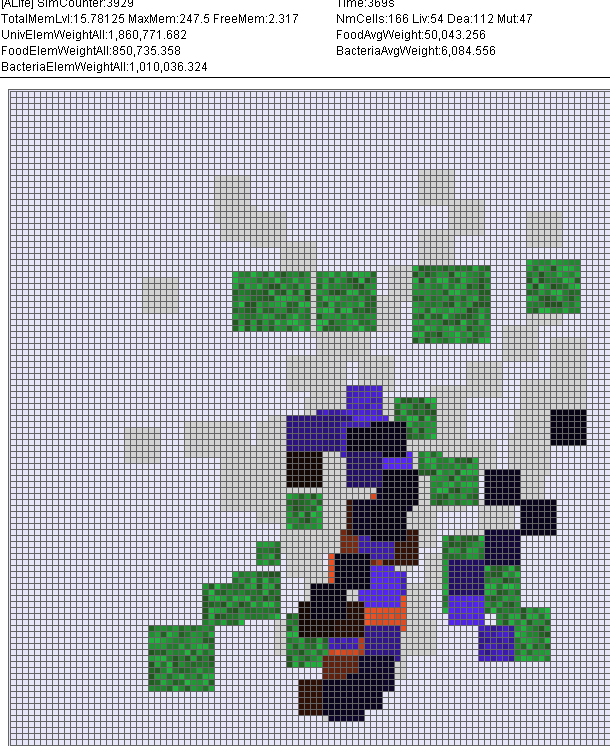
\includegraphics{moreScreenShotThruDemo}}
\caption{Code before preprocessing.}
\label{fig:one}
\end{figure}


\section{MMSN Protocol}

\subsection{Frequency Assignment}

We propose a suboptimal distribution to be used by each node, which is
easy to compute and does not depend on the number of competing
nodes. A natural candidate is an increasing geometric sequence, in
which

where $t=0,{\ldots}\,,T$, and $b$ is a number greater than $1$.

In our algorithm, we use the suboptimal approach for simplicity and
generality. We need to make the distribution of the selected back-off
time slice at each node conform to what is shown in Equation
(\ref{eqn:01}). It is implemented as follows: First, a random
variable $\alpha$ with a uniform distribution within the interval
$(0, 1)$ is generated on each node, then time slice $i$ is selected
according to the following equation:

So protocols [\citeNP{Bahl-02,Culler-01,Zhou-06,Adya-01,Culler-01};
\citeNP{Tzamaloukas-01}; \citeNP{Akyildiz-01}] that use RTS/CTS
controls\footnote{RTS/CTS controls are required to be implemented by
802.11-compliant devices. They can be used as an optional mechanism
to avoid Hidden Terminal Problems in the 802.11 standard and
protocols based on those similar to \citeN{Akyildiz-01} and
\citeN{Adya-01}.} for frequency negotiation and reservation are not
suitable for WSN applications, even though they exhibit good
performance in general wireless ad hoc
networks.

% Head 3
\subsubsection{Exclusive Frequency Assignment}

In exclusive frequency assignment, nodes first exchange their IDs
among two communication hops so that each node knows its two-hop
neighbors' IDs. 

% Head 4
\paragraph{Eavesdropping}

Even though the even selection scheme leads to even sharing of
available frequencies among any two-hop neighborhood, it involves a
number of two-hop broadcasts. To 
\subsection{Basic Notations}

As Algorithm~\ref{alg:one} states, for each frequency
number, each node calculates a random number (${\textit{Rnd}}_{\alpha}$) for
itself and a random number (${\textit{Rnd}}_{\beta}$) for each of its two-hop
neighbors with the same pseudorandom number generator.

Bus masters are divided into two disjoint sets, $\mathcal{M}_{RT}$
and $\mathcal{M}_{NRT}$.
% description
\begin{description}
\item[RT Masters]
$\mathcal{M}_{RT}=\{ \vec{m}_{1},\dots,\vec{m}_{n}\}$ denotes the
$n$ RT masters issuing real-time constrained requests. To model the
current request issued by an $\vec{m}_{i}$ in $\mathcal{M}_{RT}$,
three parameters---the recurrence time $(r_i)$, the service cycle
$(c_i)$, and the relative deadline $(d_i)$---are used, with their
relationships.
\item[NRT Masters]
$\mathcal{M}_{NRT}=\{ \vec{m}_{n+1},\dots,\vec{m}_{n+m}\}$ is a set
of $m$ masters issuing nonreal-time constrained requests. In our
model, each $\vec{m}_{j}$ in $\mathcal{M}_{NRT}$ needs only one
parameter, the service cycle, to model the current request it
issues.
\end{description}

Here, a question may arise, since each node has a global ID. Why
don't we just map nodes' IDs within two hops into a group of
frequency numbers and assign those numbers to all nodes within two
hops?

\section{Simulator}
\label{sec:sim}

If the model checker requests successors of a state which are not
created yet, the state space uses the simulator to create the
successors on-the-fly.

\subsection{Problem Formulation}

The objective of variable coalescence-based offset assignment is to find
both the coalescence scheme and the MWPC on the coalesced graph. We start
with a few definitions and lemmas for variable coalescence.

% Enunciations
\begin{definition}[Coalesced Node (C-Node)]A C-node is a set of
live ranges (webs) in the AG or IG that are coalesced. Nodes within the same
C-node cannot interfere with each other on the IG. Before any coalescing is
done, each live range is a C-node by itself.
\end{definition}

\begin{definition}[C-AG (Coalesced Access Graph)]The C-AG is the access
graph after node coalescence, which is composed of all C-nodes and C-edges.
\end{definition}

\begin{lemma}
The C-MWPC problem is NP-complete.
\end{lemma}
\begin{proof} C-MWPC can be easily reduced to the MWPC problem assuming a
coalescence graph without any edge or a fully connected interference graph.
Therefore, each C-node is an uncoalesced live range after value separation
and C-PC is equivalent to PC. A fully connected interference graph is made
possible when all live ranges interfere with each other. Thus, the C-MWPC
problem is NP-complete.
\end{proof}

\begin{lemma}[Lemma Subhead]The solution to the C-MWPC problem is no
worse than the solution to the MWPC.
\end{lemma}
\begin{proof}
Simply, any solution to the MWPC is also a solution to the
C-MWPC. But some solutions to C-MWPC may not apply to the MWPC (if any
coalescing were made).
\end{proof}

\section{Performance Evaluation}

During all the experiments, the Geographic Forwarding (GF)
\cite{Akyildiz-01} routing protocol is used. GF exploits geographic
information of nodes and conducts local data-forwarding to achieve
end-to-end routing. Our simulation is
configured according to the settings in
Table~\ref{tab:one}. Each run lasts for 2 minutes and
repeated 100 times. For each data value we present in the results,
we also give its 90\% confidence interval.

\section{Conclusions}

In this article, we develop the first multifrequency MAC protocol for
WSN applications in which each device adopts a
single radio transceiver. The different MAC design requirements for
WSNs and general wireless ad-hoc networks are
compared, and a complete WSN multifrequency MAC design (MMSN) is
put forth. During the MMSN design, we analyze and evaluate different
choices for frequency assignments and also discuss the nonuniform
back-off algorithms for the slotted media access design.

% Appendix
\appendix
\section*{APPENDIX}
\setcounter{section}{1}
In this appendix, we measure
the channel switching time of Micaz \cite{CROSSBOW} sensor devices.
In our experiments, one mote alternatingly switches between Channels
11 and 12. Every time after the node switches to a channel, it sends
out a packet immediately and then changes to a new channel as soon
as the transmission is finished. We measure the
number of packets the test mote can send in 10 seconds, denoted as
$N_{1}$. In contrast, we also measure the same value of the test
mote without switching channels, denoted as $N_{2}$. We calculate
the channel-switching time $s$ as
\begin{eqnarray}%
s=\frac{10}{N_{1}}-\frac{10}{N_{2}}. \nonumber
\end{eqnarray}%
By repeating the experiments 100 times, we get the average
channel-switching time of Micaz motes: 24.3$\mu$s.

\appendixhead{ZHOU}

% Acknowledgments
\begin{acks}
The authors would like to thank Dr. Maura Turolla of Telecom
Italia for providing specifications about the application scenario.
\end{acks}

% Bibliography
\bibliographystyle{acmsmall}
\bibliography{acmsmall-sam}

% History dates
\received{March 2011}{March 2011}{March 2011}

% Electronic Appendix
\elecappendix

\medskip

\section{This is an example of Appendix section head}

By repeating experiments 100 times, we get the average
channel-switching time of Micaz motes: 24.3 $\mu$s. We then conduct
the same experiments with different Micaz motes, as well as
experiments with the transmitter switching from Channel 11 to other
channels. In both scenarios, the channel-switching time does not have
obvious changes. (In our experiments, all values are in the range of
23.6 $\mu$s to 24.9 $\mu$s.)

\section{Appendix section head}

The primary consumer of energy in WSNs is idle listening. The key to
reduce idle listening is executing low duty-cycle on nodes. Two
primary approaches are considered in controlling duty-cycles in the
MAC layer.

\end{document}

